% Misión 5: cruzar una cueva. Portada y vuelo paso a paso.
% Centro del túnel en NED (este, norte): de la boca sur (N 10) a la norte (N 76). La columna está en
% E 9.1, N 41.9 (1.4 m a la derecha del centro): se pasa por la izquierda. Angosturas en N 26.5 y N 55.

\begin{frame}{Misión 5: cruzar una cueva}
  \begin{columns}[c]
    \column{0.56\textwidth}
    \begin{tikzpicture}
      \node[inner sep=0] (im) {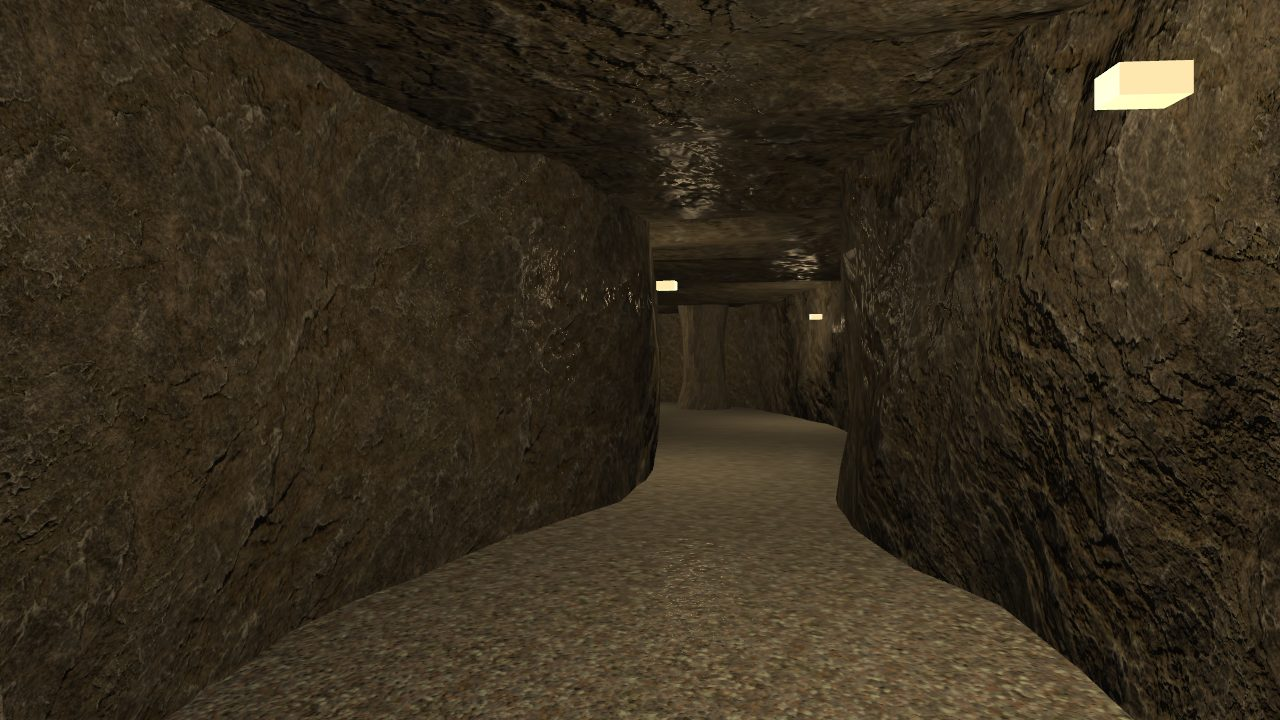
\includegraphics[width=\linewidth]{cueva_angostura}};
      \node[anchor=north west,fill=azul,text=white,font=\bfseries\scriptsize,rounded corners=2pt]
        at ([xshift=4pt,yshift=-4pt]im.north west) {MISIÓN 5 · NIVEL 2 \nivel{2}};
    \end{tikzpicture}\\[0.3em]
    \small\textbf{Escenario}: atravesar un túnel curvo de \textasciitilde66 m, con dos angosturas de 3 m y una
    columna de roca, usando \textbf{solo el lidar} para no chocar.
    \column{0.41\textwidth}
    \ficha{x500_lidar}{x500\_lidar\_2d}{cueva}{cruzar\_cueva}{\cmd{velocity\_control}}%
      {\textbf{reaccionar} a un sensor: del scan a una velocidad}{cruza, nunca a \textless 0.6 m de la roca,
      aterriza en la plataforma}
  \end{columns}
\end{frame}

\begin{frame}{La cueva, paso a paso}
  \begin{columns}[c]
    \column{0.45\textwidth}\centering
    \begin{tikzpicture}[x=0.11cm,y=0.068cm]
      \fill[gray!15] (-25,10) rectangle (25,76); \node[font=\tiny,text=gris] at (-17,70) {montaña};
      % el túnel: una franja de ~5 m alrededor del centro
      \draw[white,line width=0.55cm,smooth] plot coordinates {(0,9) (0,16) (2,23) (6,30) (8,37) (7,44) (3,50) (-1,56) (-3,63) (-2,70) (-1,77)};
      \draw[gray!50,dashed,smooth] plot coordinates {(0,9) (0,16) (2,23) (6,30) (8,37) (7,44) (3,50) (-1,56) (-3,63) (-2,70) (-1,77)};
      \fill[gray!70] (9.1,41.9) circle (1.2);
      \node[font=\tiny,right] at (11,41.9) {columna};
      \node[font=\tiny,right] at (8,26.5) {angostura};
      \node[font=\tiny,right] at (4,55) {angostura};
      \node[draw,circle,fill=azulclaro,inner sep=0.3pt,font=\tiny] at (0,0) {H};
      \fill[orange] (-2.5,82) rectangle (0.5,86);
      % recorrido
      \draw[azul,line width=1.5pt,visible on=<2->] (0,1.5) -- (0,11);
      \draw[azul,line width=1.5pt,smooth,visible on=<3->] plot coordinates {(0,11) (0,16) (1.8,23) (4,27)};
      \draw[azul,line width=1.5pt,smooth,visible on=<4->] plot coordinates {(4,27) (5.6,31) (6.6,37) (6.6,42)};
      \draw[azul,line width=1.5pt,smooth,visible on=<5->] plot coordinates {(6.6,42) (5.5,46) (3,50) (-1,56) (-3,63) (-2,70) (-1,77)};
      \draw[azul,line width=1.5pt,visible on=<6->] (-1,77) -- (-1,84);
      % el dron con sus rayos de lidar (270°, ciego atrás)
      \only<1>{\node at (0,0) {\dronarriba{0.55cm}};}
      \only<2>{\node at (0,11) {\dronarriba{0.55cm}};}
      \only<3>{\foreach \a in {-120,-100,...,120} \draw[naranja,thick] (4,27) -- ++({70+\a}:{\a>-20 && \a<20 ? 14 : 6});
        \node[rotate=-20] at (4,27) {\dronarriba{0.55cm}};}
      \only<4>{\foreach \a in {-120,-100,...,120} \draw[naranja,thick] (6.6,42) -- ++({90+\a}:{\a<-40 && \a>-100 ? 3 : 8});
        \node at (6.6,42) {\dronarriba{0.55cm}};}
      \only<5>{\node at (-1,77) {\dronarriba{0.55cm}};}
      \only<6>{\node at (-1,84) {\dronarriba{0.55cm}};}
    \end{tikzpicture}
    \column{0.53\textwidth}
    \estados{1/TAKEOFF,2/TO\_ENTRANCE,3-4/CAVE,5/TO\_PAD,6/LANDING}
    \vspace{0.3em}

    \only<1>{\begin{terminal}{ros2 launch x500\_retos cueva.launch.py}
cruzar\_cueva: esperando el lidar en /x500/scan\\
OFFBOARD activo, subiendo a 1.5 m
    \end{terminal}\small El launch levanta el puente del lidar y tu nodo. Vuela \textbf{bajito}: 1.5 m, dentro
      de un túnel de 4 m de alto.}%
    \only<2>{\begin{terminal}{cruzar\_cueva}
Arriba, yendo a la boca de la cueva\\
Dentro de la boca. De aquí en adelante, solo el lidar
    \end{terminal}\small Hasta la boca va \textbf{por posición}: afuera el lidar no ve paredes y no sabría a
      dónde ir.}%
    \only<3>{\small\textbf{Tu \cmd{steer()}}, 20 veces por segundo:
      \begin{itemize}
        \item compara izquierda contra derecha y se \textbf{centra};
        \item busca la ventana de \textpm10° \textbf{más libre} al frente y gira hacia ella;
        \item avanza más lento si tiene que girar mucho.
      \end{itemize}
      Aquí la cueva dobla a la derecha y se angosta a 3 m.}%
    \only<4>{\small\textbf{La columna}: los rayos de la derecha chocan cerca ({\color{naranja}cortos}). La ventana
      libre está a la izquierda: pasa por ahí. Si se acerca a menos de \cmd{stop\_distance} al frente, no
      avanza.}%
    \only<5>{\begin{terminal}{cruzar\_cueva}
¡Afuera! Cueva cruzada en 48 s. A la plataforma
    \end{terminal}\small Pasó la boca norte: otra vez \textbf{por posición}, a la plataforma.}%
    \only<6>{\begin{terminal}{cruzar\_cueva}
cruzó la cueva: sí OK\\
del lidar a la roca, mínimo: 1.16 m (límite 0.6) OK\\
a 0.16 m de la plataforma OK\\
Misión cumplida
    \end{terminal}}%
  \end{columns}
\end{frame}
